
\documentclass[conference]{IEEEtran}

\usepackage{cite}
\usepackage{graphicx}
\usepackage{amsmath}
\usepackage{amssymb}
\usepackage{color}
\usepackage{caption}
\usepackage{subcaption}

\graphicspath{{images/}}


% *** Do not adjust lengths that control margins, column widths, etc. ***
% *** Do not use packages that alter fonts (such as pslatex).         ***
% There should be no need to do such things with IEEEtran.cls V1.6 and later.
% (Unless specifically asked to do so by the journal or conference you plan
% to submit to, of course. )


% correct bad hyphenation here
\hyphenation{op-tical net-works semi-conduc-tor}


\begin{document}
%
% paper title
% Titles are generally capitalized except for words such as a, an, and, as,
% at, but, by, for, in, nor, of, on, or, the, to and up, which are usually
% not capitalized unless they are the first or last word of the title.
% Linebreaks \\ can be used within to get better formatting as desired.
% Do not put math or special symbols in the title.
\title{Limits of Deep Learning}


% author names and affiliations
% use a multiple column layout for up to three different
% affiliations
\author{\IEEEauthorblockN{Simon Jenni}
\IEEEauthorblockA{University of Bern\\
Email: simujenni@students.unibe.ch}
\and
\IEEEauthorblockN{Simon Brulhart}
\IEEEauthorblockA{University of Fribourg\\
Email: simon.brulhart@unifr.ch}
}


% make the title area
\maketitle

% As a general rule, do not put math, special symbols or citations
% in the abstract
\begin{abstract}
The abstract goes here.
\end{abstract}

% no keywords


% For peer review papers, you can put extra information on the cover
% page as needed:
% \ifCLASSOPTIONpeerreview
% \begin{center} \bfseries EDICS Category: 3-BBND \end{center}
% \fi
%
% For peerreview papers, this IEEEtran command inserts a page break and
% creates the second title. It will be ignored for other modes.
\IEEEpeerreviewmaketitle


\section{Introduction}

Recent state of the art natural language models represent words by embedding them
as vectors in a continuous vector space \cite{mikolov2013efficient} \cite{pennington2014glove}.
These embeddings are learned as weights of a recurrent neural network language model.
It has been demonstrated that the distributed representation of words as vectors
in a common vector-space captures not just syntactic similarities (e.g. $cat$
is close to $cats$) but semantic similarities as well. Concretely, the model's ability to
perform "word-arithmetic" has been demonstrated in \cite{mikolov2013linguistic}.
To exemplify this, let $f$ be the word-embedding function. Ideally, we would then
have an embedding where distances in vector-space give a measure of
semantic-similarity between the words. For two word pairs such as $(king:man)$
and $(queen:woman)$ which have the same relation (or similarity) we would
obtain $f(king)-f(man) = f(queen) - f(woman)$ or equivalently $f(king)-f(man) +
f(woman) = f(queen)$. This of course is equivalent to forming the analogy "$king$ is
to $man$ as $queen$ is to $woman$". 

The goal of this work is to further evaluate the performance
of the popular word2vec tool on these tasks. We evaluate the effect of
different model and learning parameters on the performance  and test
the limits of the models semantic-analysis capabilities on new challenging test data. 
The ability to learn analogies has only really been demonstrated on rather general and 
hand-picked test-sets. We test the models ability to learn domain-specific knowledge by 
generating questions that test relationships such as $Brand \thicksim Country$ 
and $Movie \thicksim Director$. Previous work only considers the nearest 
resulting vector in the embedding space when evaluating the accuracy of this word-arithmetic. 
We generalise the notion of accuracy by considering not only the nearest word-vector, but 
consider the set of the $k$ nearest vectors and test wether the target word is present therein. 


The content of this paper is structured as follows: Section \ref{sec:relwork} gives an overview 
of relevant previous work. In Section \ref{sec:model} we give a brief overview of the underlying 
model and in Section \ref{sec:exp} we outline the experimental setup and test-data used. 
The results of the experiments are then reported in Section \ref{sec:res} before we conclude
in \ref{sec:end}.


\section{Related Work}
\label{sec:relwork}

The work by Tomas Mikolov \cite{mikolov2013efficient}, where the models were introduced,
reports results on a test set they themselves created. The set contained five types of semantic
questions where relations such as $Country \thicksim Currency$ or $Country \thicksim Capitol$
were tested. In \cite{mikolov2013linguistic} the models performance on semantical
similarity has been demonstrated on SemEval-2012 Task 2 \cite{jurgens2012semeval}.
The objective in this task is to decide how similar two target word-pairs such as
$(glass:break)$ and $(soldier:fight)$ are with respect to a relation "an $X$ typically $Y$". 
Though the model is not directly trained on this task, it achieved better results than  the previous
best methods. 

In \cite{levy2015improving} Levy et. al. provide a comprehensive study of several word 
embedding techniques on the two tasks \textit{Word Similarity} and \textit{Analogy}. 
They conclude that much of the performance gains of new embedding
methods stem from design-choices and hyper-parameter optimisation rather than the 
underlying algorithms. Performance estimation was based only on the test-data sets 
introduced in \cite{mikolov2013efficient} and \cite{mikolov2013linguistic}.

In a previous work \cite{levy2014dependency} they show that generalising the Skip-Gram 
model's negative sampling to arbitrary contexts results in the model learning 
functional-similarities. They demonstrate this by manually inspecting the top $k$ most 
similar words to a given query word. A query for  \textit{Hogwarts} for example returns 
a list of famous schools in their modified Skip-Gram implementation while CBOW returns 
a list of Harry Potter characters.

\begin{figure}[t]
\centering
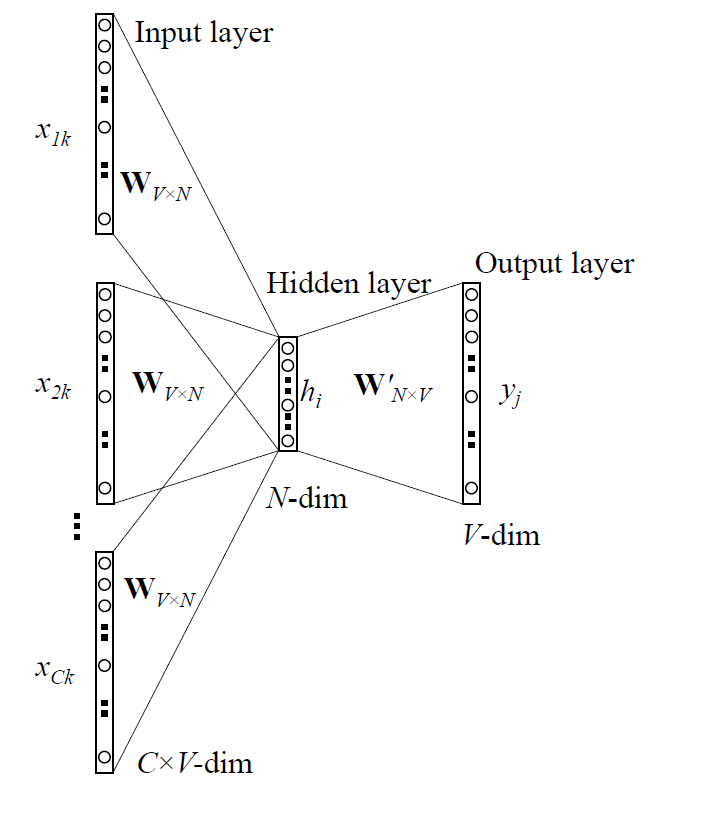
\includegraphics[width=2.5in]{cbow}
\caption{Architecture of the CBOW model. The three one-hot input vectors represent the context 
of a centre-word in a sentence and the output vector is a vector with probabilities over possible 
centre-words. }
\label{fig:cbow}
\end{figure}

\section{The Models of word2vec}
\label{sec:model}

word2vec is an implementation of the Continuous Bag of Words (CBOW) and Skip-Gram
models introduced in \cite{mikolov2013efficient}. Both of these models are based
on  two-layer recurrent neural networks with architectures depicted in Figure~\ref{fig:cbow}
and Figure~\ref{fig:skip}. The two architectures reflect the objectives of both models: CBOW
is trained to predict the centre-word from its context in a sentence while Skip-Gram tries to predict
the context from its centre. Both architectures take one-hot encoded words as inputs. Let $x_i$
denote the input corresponding to word $i$ and let the input vocabulary be $V$, 
then the inputs are given by the $|V|$-dimensional vectors:
\begin{equation}
w_{a} = \begin{pmatrix}1 \\ 0 \\ 0 \\ \vdots \\ 0 \end{pmatrix},
w_{abandon} = \begin{pmatrix}0 \\ 1 \\ 0 \\ \vdots \\ 0 \end{pmatrix}, \dots ,
w_{zone} = \begin{pmatrix}0 \\ 0  \\ \vdots \\ 0 \\ 1 \end{pmatrix}
\end{equation}

These one-hot vectors get mapped into a $N$-dimensional vector via the $|V| \times N$ weight matrix
$\boldsymbol{W}$.  The hidden unit then accumulates the sum of these vectors for all input
words in the case of CBOW and consists of only the vector associated with the single input in the 
Skip-Gram model. The output of the model is generated by multiplying the hidden-units by
weights $W'$ and applying soft-max to the result in order to generate a valid
probability-distribution over words in the vocabulary. Concretely, given a sequence of 
training words $w_1, w_2, \dots , w_T$ the hidden-states are computed as
\begin{equation}
	h(t) = \sigma (\boldsymbol{W}w(t) + \boldsymbol{H}h(t-1)),
\end{equation}
where $\boldsymbol{H}$ is the $N \times N$ matrix of hidden-to-hidden weights and 
$\sigma$ the sigmoid function:  
\begin{equation}
	\sigma (x) = \frac{1}{1+e^{-x}} 
\end{equation}
Given the values of the hidden unites, the output can be computed as 
\begin{equation}
	y(t) = P_t(\boldsymbol{W'}h(t))
\end{equation}
with the softmax function $P_t$ of a $N$-dimensional vector $x$ given by: 
\begin{equation}
	P_t(x)_i = \frac{e^{x_i}}{\sum_{j=1}^{N}{e^{x_j}}}
\end{equation}
The learnt word representation are then given by the columns of $\boldsymbol{W}$.

The models are learnt in an unsupervised fashion where either the centre-word of
a series of words is predicted from its context (CBOW) or the context is
predicted from the centre-word (Skip-Gram). Both models try to maximize the
log-likelihood of their output. Training is done via gradient descent using back-propagation
\cite{rumelhart1988learning} to compute derivatives.

At test-time when looking for the word most similar to a given word $w$ we solve for 
\begin{equation}
	x = \text{argmin}_{v \in V} d(f(w),f(v))
\end{equation}
Where $f$ is the embedding and $d$ is a distance function. We therefore search for the 
word in the vocabulary which has the minimal distance in the embedding space. The 
model as proposed by \cite{mikolov2013efficient} chose $d$ to be the cosine-distance, 
but we investigate different choices such as $L^p$- or Dice-norms.

\begin{figure}[t]
\centering
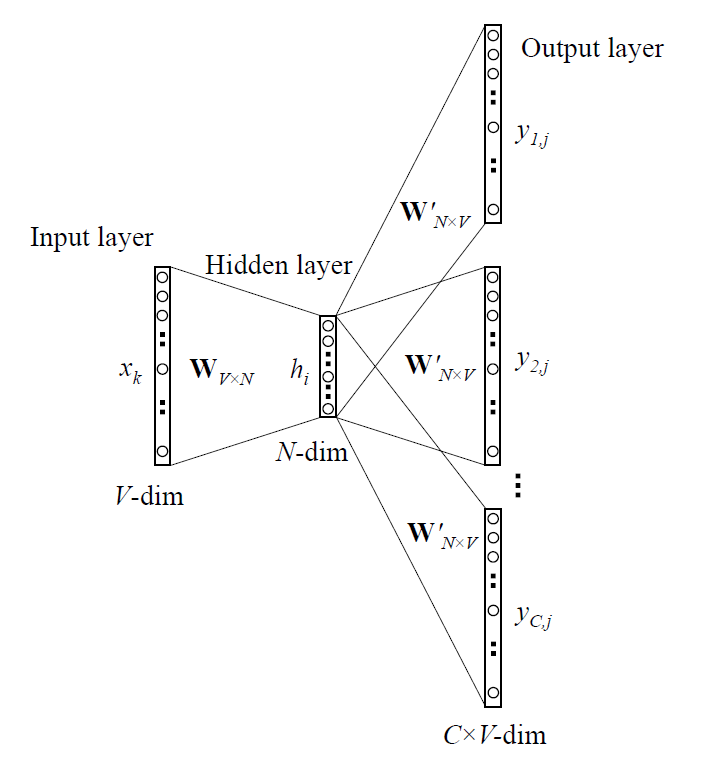
\includegraphics[width=2.5in]{skip-gram}
\caption{Architecture of the Skip-Gram model. The output of this model are vectors with probabilities 
for the words occurring in the context of the input word.}
\label{fig:skip}
\end{figure}


\section{Experiments}
\label{sec:exp}

In this sections we first outline our experimental setup, introduce novel test-data
 and then report results obtained for different hyper-parameter choices and test scenarios. 

\subsection{Setup}
We used the Python re-implementation of word2vec contained in the Gensim library 
\cite{rehurek_lrec}. This implementation is functionally identical to the original 
C-implementation provided by \cite{mikolov2013efficient}, but is more readable and has 
shown to perform just as well. 

To compare the influence of hyper-parameters on the performance we train several models
with different values for one of the parameters and keep all other parameters fixed. We 
identified the following set of hyper-parameters for our experiments:
\begin{enumerate}
\item Context-window size
\item Vector size (i.e dimension of hidden-layer)
\item Learning rate $\alpha$
\item Training corpus
\item Hierarchical softmax vs. negative sampling for Skip-Gram
\end{enumerate}


\subsection{New Test Data}
To test the models performance on domain-specific questions we constructed several 
question sets. The questions are all of the form "X is to Y as U is to ?", i.e. they take the 
form of analogies. We constructed the following sets of questions:

\subsubsection{Brand-Origin}
A set of questions testing for the relationship between well-known brands and their countries
of origin. To construct this question-set we gathered names and country of origin for 
the top 500 brands according to brandfinance.com. We excluded all the brands from countries
with names consisting of multiple words (e.g. United States of America,...) due to the model 
working on single words. The result if a set of 38'220 questions.

\subsubsection{Movie-Director}
A set of analogy-questions for the relationship between famous movies and their respective 
directors. The set was constructed by gathering movie-titles and last-name of the director for 
some of the top rated movies according to IMDb. Similar to the Brand-Origin questions we 
excluded movies with titles consisting of more than one word with the exception of titles 
starting with "The ..." or similar.  The result if a set of 4'557 questions. 


\subsection{Results}
\label{sec:res}




% An example of a floating figure using the graphicx package.
% Note that \label must occur AFTER (or within) \caption.
% For figures, \caption should occur after the \includegraphics.
% Note that IEEEtran v1.7 and later has special internal code that
% is designed to preserve the operation of \label within \caption
% even when the captionsoff option is in effect. However, because
% of issues like this, it may be the safest practice to put all your
% \label just after \caption rather than within \caption{}.
%
% Reminder: the "draftcls" or "draftclsnofoot", not "draft", class
% option should be used if it is desired that the figures are to be
% displayed while in draft mode.
%
%\begin{figure}[!t]
%\centering
%\includegraphics[width=2.5in]{myfigure}
% where an .eps filename suffix will be assumed under latex,
% and a .pdf suffix will be assumed for pdflatex; or what has been declared
% via \DeclareGraphicsExtensions.
%\caption{Simulation results for the network.}
%\label{fig_sim}
%\end{figure}

% Note that the IEEE typically puts floats only at the top, even when this
% results in a large percentage of a column being occupied by floats.


% An example of a double column floating figure using two subfigures.
% (The subfig.sty package must be loaded for this to work.)
% The subfigure \label commands are set within each subfloat command,
% and the \label for the overall figure must come after \caption.
% \hfil is used as a separator to get equal spacing.
% Watch out that the combined width of all the subfigures on a
% line do not exceed the text width or a line break will occur.
%
%\begin{figure*}[!t]
%\centering
%\subfloat[Case I]{\includegraphics[width=2.5in]{box}%
%\label{fig_first_case}}
%\hfil
%\subfloat[Case II]{\includegraphics[width=2.5in]{box}%
%\label{fig_second_case}}
%\caption{Simulation results for the network.}
%\label{fig_sim}
%\end{figure*}
%
% Note that often IEEE papers with subfigures do not employ subfigure
% captions (using the optional argument to \subfloat[]), but instead will
% reference/describe all of them (a), (b), etc., within the main caption.
% Be aware that for subfig.sty to generate the (a), (b), etc., subfigure
% labels, the optional argument to \subfloat must be present. If a
% subcaption is not desired, just leave its contents blank,
% e.g., \subfloat[].


% An example of a floating table. Note that, for IEEE style tables, the
% \caption command should come BEFORE the table and, given that table
% captions serve much like titles, are usually capitalized except for words
% such as a, an, and, as, at, but, by, for, in, nor, of, on, or, the, to
% and up, which are usually not capitalized unless they are the first or
% last word of the caption. Table text will default to \footnotesize as
% the IEEE normally uses this smaller font for tables.
% The \label must come after \caption as always.
%
%\begin{table}[!t]
%% increase table row spacing, adjust to taste
%\renewcommand{\arraystretch}{1.3}
% if using array.sty, it might be a good idea to tweak the value of
% \extrarowheight as needed to properly center the text within the cells
%\caption{An Example of a Table}
%\label{table_example}
%\centering
%% Some packages, such as MDW tools, offer better commands for making tables
%% than the plain LaTeX2e tabular which is used here.
%\begin{tabular}{|c||c|}
%\hline
%One & Two\\
%\hline
%Three & Four\\
%\hline
%\end{tabular}
%\end{table}


% Note that the IEEE does not put floats in the very first column
% - or typically anywhere on the first page for that matter. Also,
% in-text middle ("here") positioning is typically not used, but it
% is allowed and encouraged for Computer Society conferences (but
% not Computer Society journals). Most IEEE journals/conferences use
% top floats exclusively.
% Note that, LaTeX2e, unlike IEEE journals/conferences, places
% footnotes above bottom floats. This can be corrected via the
% \fnbelowfloat command of the stfloats package.




\section{Conclusion}
\label{sec:end}

The conclusion goes here.




% conference papers do not normally have an appendix



% trigger a \newpage just before the given reference
% number - used to balance the columns on the last page
% adjust value as needed - may need to be readjusted if
% the document is modified later
%\IEEEtriggeratref{8}
% The "triggered" command can be changed if desired:
%\IEEEtriggercmd{\enlargethispage{-5in}}

% references section

% can use a bibliography generated by BibTeX as a .bbl file
% BibTeX documentation can be easily obtained at:
% http://mirror.ctan.org/biblio/bibtex/contrib/doc/
% The IEEEtran BibTeX style support page is at:
% http://www.michaelshell.org/tex/ieeetran/bibtex/
\bibliographystyle{IEEEtran}
% argument is your BibTeX string definitions and bibliography database(s)
\bibliography{IEEEabrv,./bibliography}




% that's all folks
\end{document}
